% #############################################################################
% This is Chapter 2
% !TEX root = ../main.tex
% #############################################################################
% Change the Name of the Chapter i the following line
\fancychapter{State of the Art}
\cleardoublepage
% The following line allows to ref this chapter
\label{chap:back}

In this section, a state-of-the-art analysis will be made to the current literature and technologies regarding the main subjects of this thesis. These will encompass the existing projects and sensors for the measurement of air quality, specifically regarding PM, the \ac{LPWAN} IoT technologies and hardware platforms used along with these in remote systems development, the current SIMs and algorithms used for environmental phenomena estimation and visualization, and finally, the current available solutions at public disposal for the visualization of live air quality, in the form of web applications.

% #############################################################################
\section{PM Measurement}

There are many types of instruments and methods for the measurement of the concentration and size distribution of PM. These rely on the various behavior characteristics of particles (mobility, aerodynamics and diffusion) \cite{Amaral2015}. The scope of this thesis only encompasses the measurement of the concentration of PM10 and PM2.5, due to its harm to human health, reviewed in the previous chapter, therefore no size distribution methods will be described. 

The main methods for the measurement of PM concentration in ambient air are gravimetric, optical and microbalance \cite{Amaral2015}.


\subsection{Gravimetric}

The gravimetric method is the European reference method for sampling and determining PM10 and PM2.5 in ambient air, as in the norm EN 12341:2014. 

In the gravimetric method, particle mass concentration is determined through the usage of filters to weigh particles, before and after the sampling period. It is considered as the basic method to measure PM mass concentrations in combustion gases. The filter collects PM in all granulometric fractions and sizes and then a cyclone or impactor is used to remove larger particles. These filters can only output measures from 15 to 15 minutes, therefore this method is not ideal for the identification of real time events. However, the collected particles can be analyzed chemically, which is not possible in some of the other methods.
The filters used in this method are very condition and calibration dependant \cite{Amaral2015}. 

%In Figure XX is presented an example of a reference high-volume gravimetric sensor equipment, Sierra-Andersen


\subsection{Optical}

Optical instruments can be based on the principles of light scattering, absorption or extinction, with scattering being the most usual. They usually include dispersion photometers for the measurement of the intensity of scattered light in one or more angles from a combination of all the particles present in the optical detection volume. 
In the light scattering methods, particles are hit by a light beam and irradiate that light in every direction.
Most commercial light scattering instruments use visible light and measuring angles of 90°, 45°, or less than 30° \cite{Amaral2015}.


\subsection{Microbalance}

In the microbalance method, particles are collected into the surface of an oscillatory microbalance, then through oscillation, these use the alteration of resonance frequency to determine PM concentration.
For this method there are two main prevalent instruments, the Tapered Element Oscillation Microbalance and the Quartz Crystal Microbalance.

In the first one, PM mass is measured based on the alteration of resonance frequency of a tapered quartz wand, according to the accumulation of particles in a sampling filter, connected to the wand. In the second, the quartz crystal has a piezoelectric property of changing its resonance frequency when there is a small addition of mass in its surface, with particles being deposited by electrostatic precipitation in a fine quartz
crystal resonator, instead of a sampling filter \cite{Amaral2015}.

Amaral et al., in 2015, reviewed every type of PM instrument available in the market, with the goal of helping researchers choose the most suitable equipment for their application. It was concluded that when deciding which device is most appropriate, issues such as detection limit and size range of the instrument must be evaluated \cite{Amaral2015}. 

Regarding specific instruments, it was concluded that methods which use filters are not very accurate, but have the advantage of performing chemical analysis in the measured particles. It also requires a lot of labor for it to function properly. Finally, it is also concluded that there was not an absolute best instrument for measuring PM, but a most suitable for each situation, and that different methods should simultaneously be used, in order to confirm values during sampling.


\subsection{Portuguese Monitoring Station Network}

In \Cref{fig:apa-stations-location} is presented the current monitoring network in the county of Lisbon presented in QualAr website, where it is possible to see the available stations at a certain time, along with color graded measures from the available stations \cite{QualAr}.
In Portugal, according to the Manual on Methods and Operational Procedures of Air Quality Monitoring Networks, made by the Portuguese Environmental Reference Laboratory, the methods used for the measurement of PM10 and PM2.5 are the gravimetric and the beta ray absorption \cite{LaboratoriodeReferenciadoAmbiente2010}.

The gravimetric method works as stated in Section 2.1.1. It allows determining the mass of particles deposited in the filters, and these are later used in laboratory to determine particle chemical properties \cite{LaboratoriodeReferenciadoAmbiente2010}.


The monitor used at the stations at the time of this thesis, which was used as reference in this work, was the Environnement S.A. Model MP101M, which is certified equivalent to the reference method in accordance with the EN12341 European standards for PM10 and PM2.5 particulate concentration. It is based on the beta ray attenuation measurement technique, which is an optical light absorption PM concentration measurement method \cite{environnementSA}.

A schematic summary of every PM concentration measurement method analysed in this section is presented in \Cref{fig:pm-measurement-methods}.

\begin{figure}[ht]
\centering
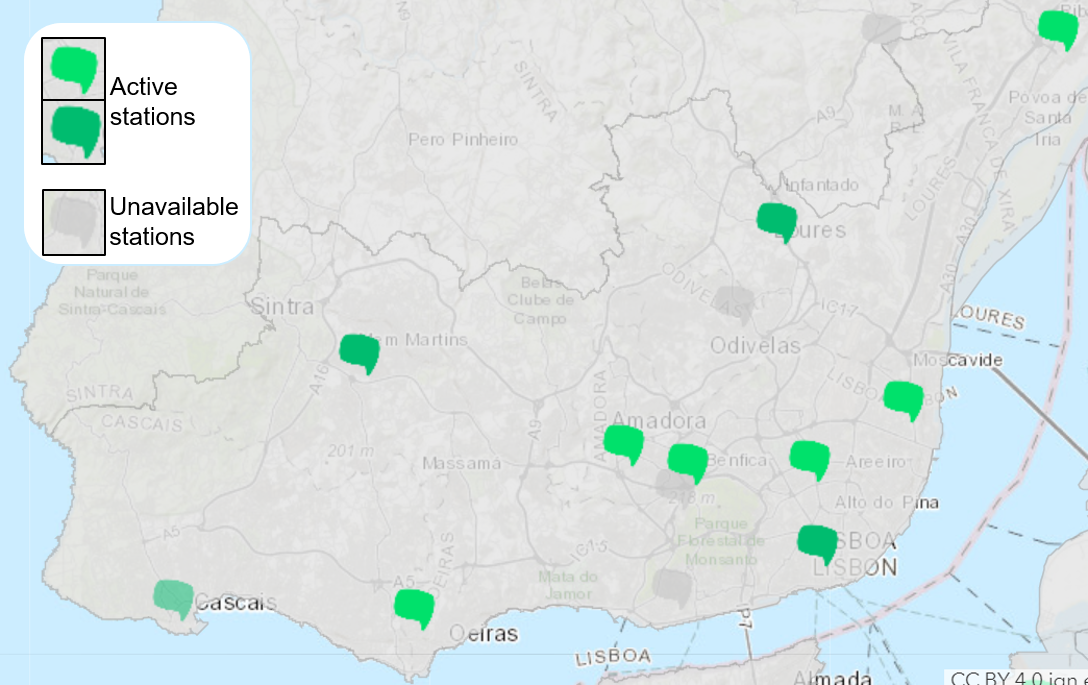
\includegraphics[width=0.8\textwidth]{./Images/apa-stations-location.PNG}
\caption{Current monitoring network in the county of Lisbon.}
\label{fig:apa-stations-location}
\end{figure}

\begin{figure}[ht]
\centering
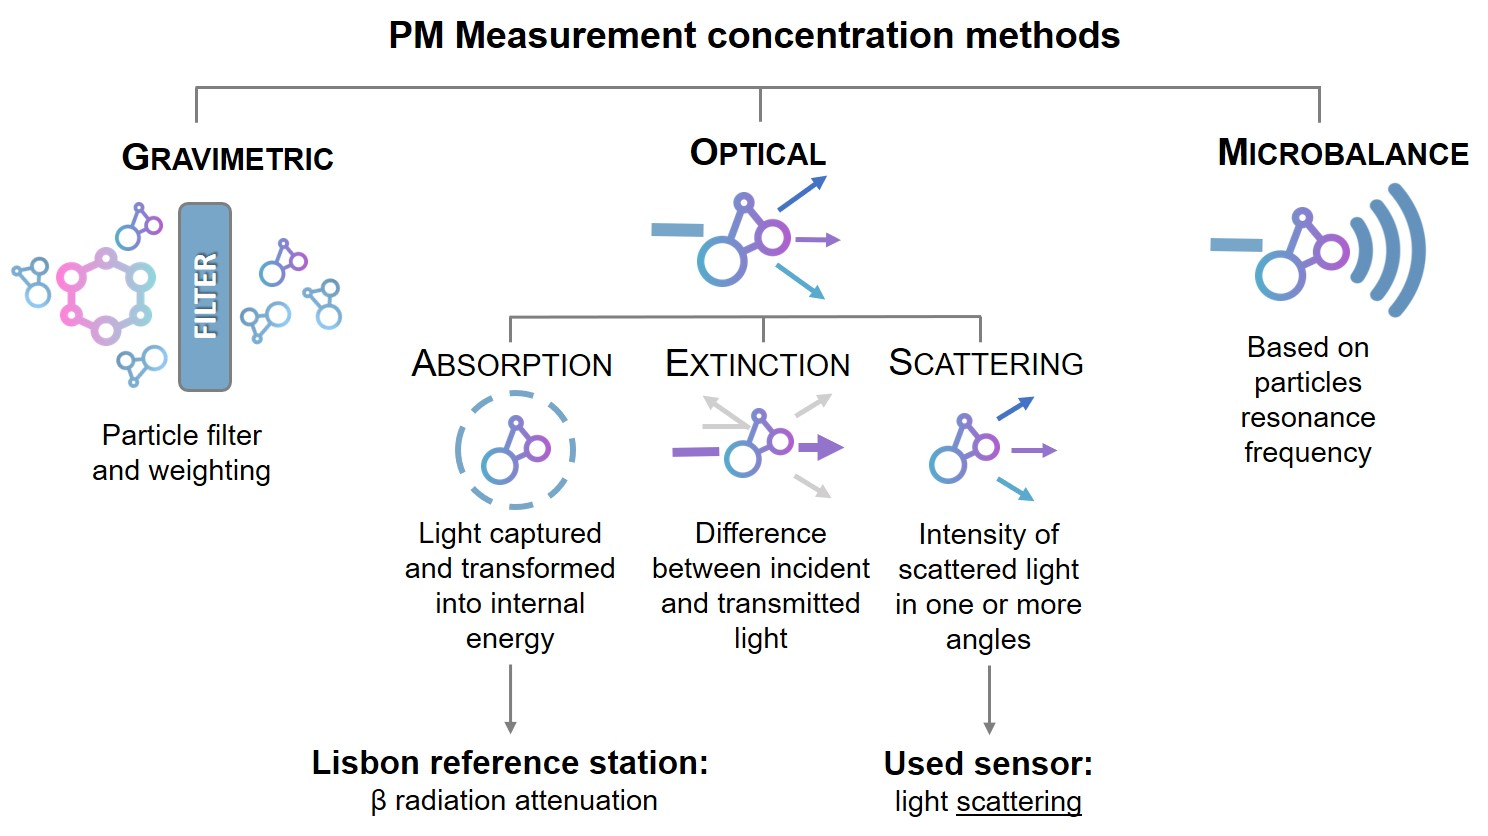
\includegraphics[width=0.9\textwidth]{./Images/pm-measurement-methods.jpg}
\caption{PM concentration measurement methods.}
\label{fig:pm-measurement-methods}
\end{figure}

% #############################################################################
\section{Low-cost Air Monitoring Systems}

The scope of this thesis is aimed at the usage of low-cost sensors to further extend current monitoring networks with more data. For this to work, some examples of usage of low-cost sensors were observed in the literature in order to conclude whether these low-cost PM sensors are reliable, taking into account its performance, cost, and calibration needs.

Several models for monitoring systems have been developed with the objective of providing a better solution for the monitoring of air pollution with much lower maintenance and production costs than the current monitoring stations. Many of these use IoT devices and take advantage from mobile communication technologies \cite{Zheng2018}\cite{Wendt2019}\cite{Quelhas2011}. 

In this section, first there will be an overview over research projects and dissertations prior to this thesis where air quality was attempted to be measured at low-costs. Second, it will be shown literature regarding the performance of low-cost PM sensors currently available in the market.

\subsection{Previous Projects}

In 2008, Carvalho developed, in his thesis, a mobile system to monitor air quality which could be connected to mobile objects such as a bus or a taxi, in order to acquire a map of the quality of air \cite{Carvalho2008}. This system had a \ac{GPS} module to provide the location of the system and a \ac{GSM} module to transmit data to a central server. The measured gases were CO, NO2, O3, SO2 and CO2, therefore PM measures were absent. Each module was self-sufficient and supplied by solar panel charged batteries, and the gases measures were presented in the server in a numerical or geographical form overlapped with a map of the city of Lisbon. However not many campaigns were done, with not much data being collected, and the system's sensors were not calibrated with the reference standard measuring stations. 

In 2011, in the context of an improvement of air quality project named URBISNET, which took place in Lisbon, made by several researchers from Instituto Superior Técnico, a prototype of a mobile station for air quality mapping sensor network was developed \cite{Quelhas2011}. This prototype also measured many polluting gases, used GPS, significant processing power, data storage, many inputs and outputs for the different sensors, and GSM. Despite the efforts on the development of this solution, there were problems with the calibration and overall validation of some of the low-cost gas sensors, which rendered the prototype not very useful and with relatively high production costs for the functions provided.

Vehicle and Propulsion Systems Laboratory, currently operating in Instituto Superior Técnico, in its proposal of creation, with the coordination of Tiago Farias, proposed a project for monitoring pedestrians exposure to PM \cite{Farias2013}. This consisted of a 11 kg bag, with a GPS module, a micro-controller, a particulate and dust sensor, a numerical pad and a computer. The collection of particle concentration data combined with nearly instant measures and the live GPS monitoring allow the estimation of the pollution pedestrians are exposed to throughout certain routes.

\subsection{Low-cost PM sensors}

Low-cost solutions for PM measurement currently in the market consist mostly of optical instruments. These are made of small lasers placed in an certain angle, against a photodiode, which is used to detect the scattered light of illuminated particles, as stated in Section 2.1.2. The generated light scattering signal is filtered and amplified. Afterwards a modulation signal is used to represent the measurements. These sensors usually cost less than 50 euros, which is a considerable difference in relation to reference instruments, which have much more expensive production and maintenance costs.

Despite their price, low-cost optical PM monitors can be used to characterize PM concentrations with high spatial and temporal resolution \cite{Manikonda2016}. In 2016, Manikonda et al. conducted a study with the objective of assessing these monitors and concluded that they perform with adequate precision for indoor air monitoring, although with some calibration requirements \cite{Manikonda2016}. Currently, many professional small factor air quality monitoring stations, for both indoor and outdoor applications, are available in the market. Additionally, communities have been formed with the objective of creating networks where individuals can collect and share data from their personal monitoring systems so that all the obtained data is presented collectively in a map. An example of this is the Weather Underground community \cite{WeatherUnderg2019}.

Some of these monitoring stations are known to use low-cost and compact size light-scattering based PM sensors, namely, the stations manufactured by Gaia Earth Sensing Labs, which use specifically Plantower PMS sensors \cite{AQICN}. These manufacturers have many product variants for outdoor monitoring. One of these products is presented in \Cref{fig:ieec3}.

\begin{figure}[ht]
\centering
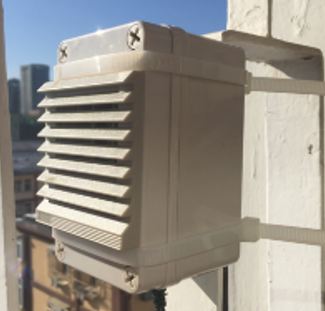
\includegraphics[width=0.4\textwidth]{./Images/ieec3.png}
\caption{Example of commercialized PM monitors.}
\label{fig:ieec3}
\end{figure}

A study from the University of Utah, in 2018, performed a long-term field evaluation of the Plantower PMS sensors, in which for 320 days, multiple season variations, and significant PM2.5 variation events, measurements were undertaken by two sensors, PMS5003 and two PMS1003, with tracking made through co-located reference air monitors. The results of this study demonstrated overall good correlations between the PMS sensors and reference monitors in the winter season, seasonal differences in sensor performance, some intra-sensor variability, and drift in one sensor, with worse results associated to the PMS1003 sensor \cite{Sayahi2018}.


Kuula et al., in 2019, investigated how sensors can be used in urban areas to complement existing air quality networks, through a campaign during the winter, with the use of the optical sensors PPD60PV and PPD42NS. These were also compared to reference instruments \cite{Kuula2019}. The results showed that these sensors could measure PM10 and PM2.5 with reasonably high correlations. It was concluded that comprehensive understanding of the sensor characteristics is necessary, and that the sensor must be validated and calibrated in the environment where it will be placed. It is also stated that one big disadvantage of these sensors is the non-guaranteed accuracy and the lack of established scientific literature. Results also show that optical sensors are suitable for measuring mass concentrations of particles that are larger than 0.5 $µm$, and that diffusion charging based sensors, instruments which use light extinction to monitor particle concentrations, are better for traffic exhaust and local combustion related ultra fine particles.

Despite being promising, the performance of these low-cost PM sensors under field conditions is still not well understood. In order to characterize the performance capabilities of a low-cost PM sensor, PMS3003 from Plantower, Zheng et al., in 2018, performed a study where these sensors were tested in both low and high particle concentration regions, during different seasons, to determine how the sensors perform across a range of concentrations and meteorological factors \cite{Zheng2018}. The attained results showed that \ac{RH} has a major influence in the sensor measures, while the temperature effects were negligible. With that, calibration correction factors were applied to measures taken by the sensor, and the mean errors were reduced from 27\% to 10\% at different time resolutions, when compared to high precision reference instruments. After calibration, the results proved that the sensor can be a promising addition to current PM sensor networks.

The South Coast Air Quality Management District, agency responsible for South California air quality monitoring, in 2018, field-tested Plantower PMS5003 PM sensor, and notable correlation and precision was attained between the PMS5003 and the reference instruments \cite{AQ-SPEC}.


% #############################################################################
\section{Interpolation Algorithms for Spatial Analysis}

Air quality analysis relies in mathematical approaches to explain the polluting gases concentration evolution. The process of developing this type of prevision with high spatial resolution is a rather complex problem, due to the wide sources of pollution in urban and industrial areas, and to all the variables that can influence air quality.

Approaches to this problem in the literature are sometimes deterministic, which require a lot of knowledge on the local sources and factors that can influence air pollution, or otherwise rely on measurement data. Spatial interpolation consists in estimating the value of measures of certain properties, at unsampled locations, within the area covered by existing observations of the same properties. The objective is to present a much more detailed overview of the air quality in a certain region.

Currently, SIMs are well developed and frequently used in various \ac{GIS} applications, in which they can be used to manipulate, analyze and present data in spatial representations. Spatial interpolation is based on the fact that observation points that are closer to each other have more similarities than the ones far away, which is known as Tobler’s First Law of Geography \cite{Stein1994}.

Some of the most popular and standardized SIMs, since the beginning of spatial interpolation modeling, are \ac{IDW}, kriging, shape functions, spline, and trend surface. These occur from different approaches to this problem, such as local neighborhood, geostatistical and variational \cite{Li2008}.

In 2014, Li and Heap made a review of the 25 most commonly applied SIMs \cite{Li2014}. As result an easy to use decision tree was created for use case dependent method selection. According to it, the most suitable interpolation algorithms in circumstances such as the ones in this work are IDW and \ac{OK}, depending on data selection and availability.

\subsection{Fuzzy Boolean Networks}

FBNs are boolean networks developed and studied by researchers at Instituto Superior Técnico \cite{Tome}. 
In order to correctly explain the functioning of these, a proper nomenclature needs to be given to its constituents.

The networks are constituted by neuronal areas. Each area has a set of neurons, and the number of neurons, which is user defined, must be equal in all areas. Each neuron has a binary value and is constituted by a binary table with a user defined length. The value at each index of each table is considered a memory of the respective neuron, and all memories are initialized with a random number between zero and one. The number of memories of each consequent neuron is equal to a granularity factor.

Each neuronal area can only be one of two types, antecedent or consequent, with their corresponding neurons named after the area, antecedent or consequent neurons respectively. FBNs must have at least one neuronal area of each of the two types. In these networks, connections are weightless, temporary, circumstance dependent and only appear between neurons located in different areas of different types, either in the learning or in the inference process.
In \Cref{fig:fbn-drawing} a very simple example of an FBN is presented, with  two antecedent areas and one consequent area, each with four neurons. The granularity factor is two and consequently, neurons in the consequent area have four memories each. In this representation dark neurons have the value one, and white neurons have the value zero.

\begin{figure}[ht]
\centering
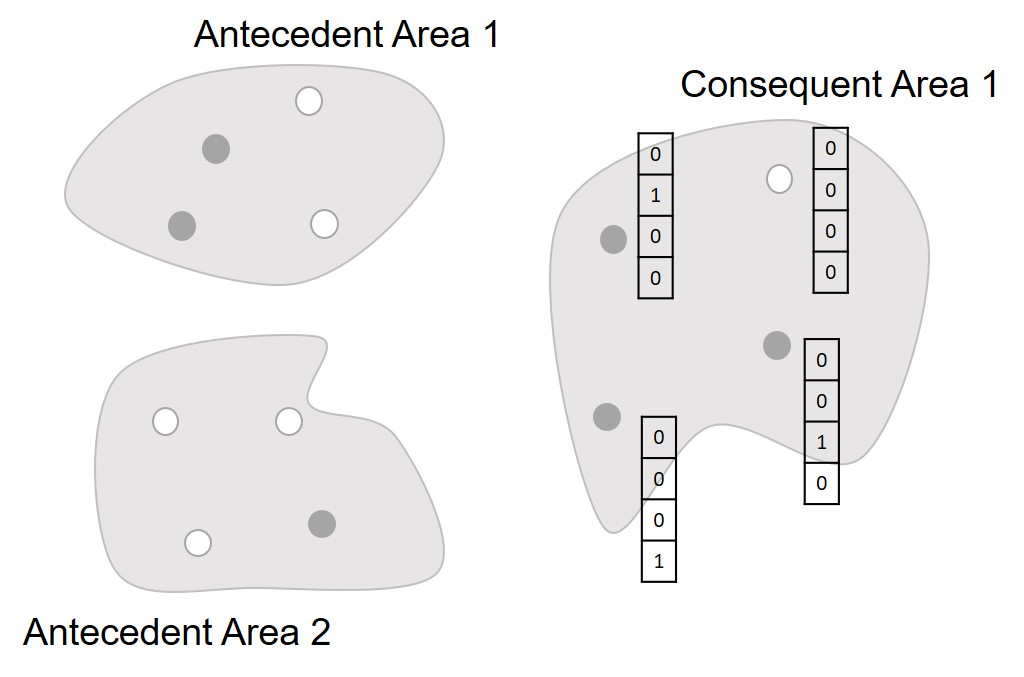
\includegraphics[width=0.65\textwidth]{./Images/fbn-drawing.jpg}
\caption{Example of the constituents of a FBN.}
\label{fig:fbn-drawing}
\end{figure}

In what regards the usage of these networks, the number of areas is defined by the number of variables in the problem. To each independent variable, an antecedent area is created and associated. The same happens with the dependent variables, for which consequent areas are created and respectively associated. As an example of usage, if used for linear interpolation, the FBN would only have an antecedent area, associated to the x axis (independent), and a consequent area, associated to the y axis (dependent). The network represented in \Cref{fig:fbn-drawing} has two independent and one dependent areas, being the latter the subject of inference.

Before the creation of the network, the definition of its parameters must be made. These parameters are the size of each neuronal area, the number of memories per neuron, the granularity factor and the number of samples each neuron uses in the inferring and learning processes. Each should be previously tested and assessed comparatively by the researcher, to each different use case \cite{Tome2014}.

The learning process of these networks is composed of several phases:
\begin{itemize}
\item First, for each network there will be sets of values of each variable in the problem. These are considered the rules that the network will learn. For each set, and for each variable, its value is translated into a percentage. Each corresponding area will be activated according to this percentage, that is, the neuron values for that area will be 1 with the probability of that percentage, and rest will remain at zero.
\item Second, each neuron, in the consequent areas, samples an user defined number of neurons from each antecedent area. This number must always be the same for every neuron and antecedent area, and counts the number of one valued neurons for each area. 
\item For each count that neuron attained, it multiplies that count by the granularity factor raised to the power of the number of the antecedent area of the respective count.
\item Finally, each consequent neuron stores its own binary value (which was defined during the consequent area initial activation) in its memory table, in the index corresponding to the previously acquired count.
\end{itemize}

Various iterations of this process, for different training values for every variable,  represent how training is performed in FBNs.
Assuming each memory was initialized with the value zero, it is possible that the represented FBN has already been trained with exactly one set of values, since one memory per activated consequent neuron has the value of one. In this single learning process step, one could conjecture that the connections for that step were as portrayed in \Cref{fig:fbn-drawing-2}, according to the activated indexes of the table of memories of each consequent neuron (connections with the zero valued neuron in the consequent area were not placed in the figure for ease of visualization, since they are not relevant).

\begin{figure}[ht]
\centering
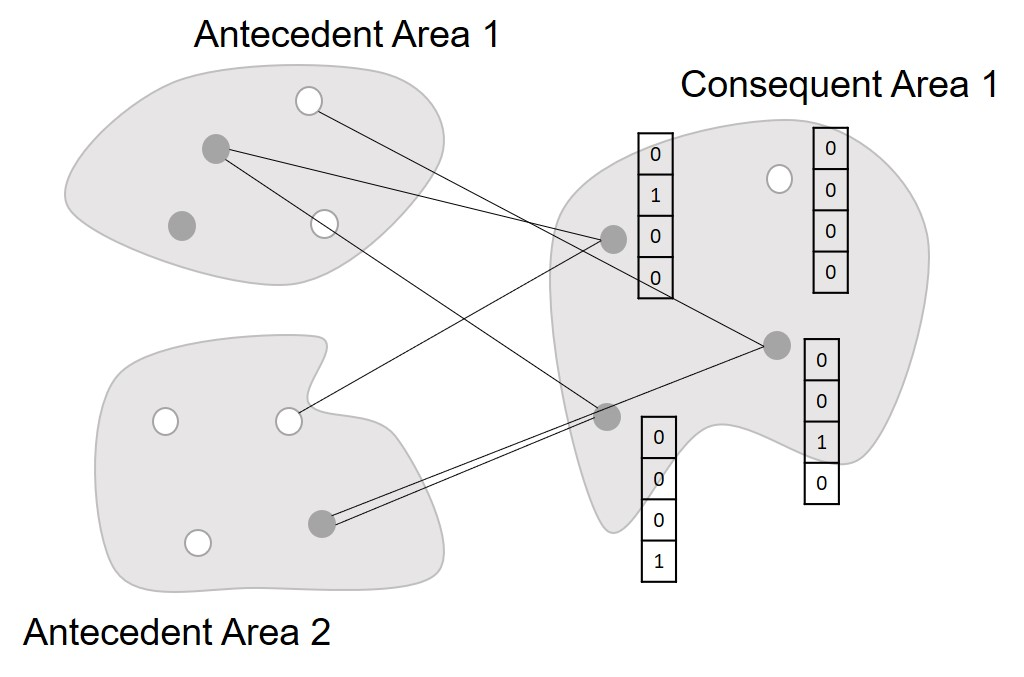
\includegraphics[width=0.65\textwidth]{./Images/fbn-drawing-2.jpg}
\caption{Example of the learning process of a FBN.}
\label{fig:fbn-drawing-2}
\end{figure}

In the inference process, the network only receives the value of the independent variables and it is supposed to infer the dependent variables value:
\begin{itemize}
\item Initially, only the antecedent areas are activated according to its variables value translated into percentage. 
\item Afterwards, in the exact same fashion of the learning process, every consequent neuron performs sampling, ending up with a count for each antecedent area. The value in the corresponding memory of that neuron is verified. If it stores a zero, then that neuron value will be modified to zero, if it stores a one, its value will be modified to one.
\item In the end of this process every neuron in every consequent area will have a binary value. Therefore, consequent areas can be translated into a percentage according to its activation ratio. 
\item This percentage is translated into the scale of the corresponding dependent variable, and it represents the inference value for the respective variable, in the respective set, according to the respective learning rules.
\end{itemize}

Studies have concluded that these networks have many nature and biologic like characteristics, such as the organization of neurons per area, to which a given variable or concept can be associated. They have random individual connections and structured meshes of links between them. They are also characterized by relative noise immunity and the capability to approximate reasoning and learning. Provided the remaining neurons are enough to define activation ratios accurately, any number of neurons or connections may be deleted or corrupted \cite{Tome2014}.

It has also been shown that the FBN learning process converges for a repetitive sequence of different rules, where in the limit, the system is able to learn a number of rules compatible with a granularity that increases with the square root of the number of inputs per neuron and per antecedent \cite{Carvalho2002}.

As Universal Approximators, FBN can learn multi-input single-output functions, and they perform pretty well in comparison to other techniques when parametrization is rather difficult. FBN perform better when the training data is very sparse, and data-sets are imbalanced \cite{Carvalho2007}. They are shown to be immune to individual neuron or connection errors, which does not happen with \ac{ANN}, and also have good generalization capabilities \cite{Carvalho2007}.
However, one problem that arises from the use of FBN is the that the memory necessity increases exponentially with the number of inputs and size of the network, which is a notable limiting factor.

Tomé et al., in 2014, in a deep analysis of FBN, despite assessing its main characteristics and advantages, also made experiments in which learning, and interpolation capabilities were compared, by interpolating sparse data. The comparisons were made between FBN, \ac{ANFIS}, ANN, Cubic spline interpolation, Support Vector Machines and Isotonic Regression Model, and it was shown that FBN outperformed all other interpolation algorithms. Even when used as a classifier, FBN outperformed every other algorithm, given a sparse set of data \cite{Tome2014}.

\subsection{Inverse Distance Weighting}

IDW is a deterministic SIM based on the assumption that the degree of influence of the nearby sample points should be greater than the effect of more distant points. Its maximum and minimum value can not occur outside the sampled points. The only parameter which is user defined in the IDW implementation is the power function, which defines the relevance of the distance to the weights of each observed value \cite{Mesquita2009}.

The IDW interpolation can be defined by the equation \eqref{idw}, where \eqref{idw-weight} represents the weights associated to each observation.

\begin{equation} 
\label{idw}
\scalebox{1.4}{ $ f(x, y) = \dfrac{\sum_{i=1}^{n} w(d_i)z_i}{\sum_{i=1}^{n} w(d_i)}, i = 1, 2, ..., n$}
\end{equation}

\begin{equation} 
\label{idw-weight}
\scalebox{1.3}{ $w(d_i)= \dfrac{1}{{d_i}^{p}}$}
\end{equation}

Where $z_i$ is the observed value, $d_i$ is the distance between the estimation and the observation points, $w(d_i)$ represents the weight associated to observation \textit{i}, and \textit{p} is the power function.

In IDW, weights are proportional to the inverse of the distance elevated to the power of p. Therefore, as distance increases, weights decrease, in a rate that increases the higher the value of p.
When p is zero, the resulting estimate is simply equal to the spatial average of all sampled points.
%The IDW can be either global or local and exact or gradual.

Even though IDW is one of the most widely used interpolation models, it has several limitations, such as its inability to produce error statistics, unlike OK, and the fact that spatial relationships between two locations are not only dependent on distance neither are they constant over space \cite{Mesquita2009}.

\subsection{Kriging}

Kriging interpolation models are fundamental geostatistic tools in the field of spatial analysis.

The main difference between kriging and other non-geostatistical models is the assumption that the spatial correlation structure of the process under study is known and can be estimated from the observed data. In kriging, weights are based not only in the distance between points but also in the overall spatial arrangement of observation points \cite{Mesquita2009}.

The kriging schemes are stochastic, local, gradual and exact interpolators. Its methodology includes two stages: the analysis of the spatial variation and the estimation of the target variable, which is also based on the weighted average approach. Furthermore, it uses several statistic models which allow the construction of a variety of maps, including previsions, errors of previsions and probabilities, which are considerable advantages in comparison to IDW.

Before kriging is used, an exploratory statistical analysis of data must be made, as well as the modelling of a variogram to represent how semivariance varies with distance. The analysis of the spatial variation is performed through the variogram modelling of how distance variations with semivariance are not linear, but have a custom relation. In \Cref{fig:variogram}, an example of a variogram is presented. The nugget represents the semivariance value when the distance tends to zero. The sill is the point where semivariance stabilizes, and range is the interval in which as distance increases, higher is the semivariance. Kriging interpolation weights are chosen using the modeled variogram, so that estimates are unbiased and the estimation variance is minimized.

The most common kriging models are simple kriging, which assumes a known constant mean, OK, which assumes that there is an unknown constant mean, estimated from the data and universal kriging, which assumes that there is a trend in the surface that partly explains the data variations \cite{Deligiorgi2011}.

\begin{figure}[ht]
\centering
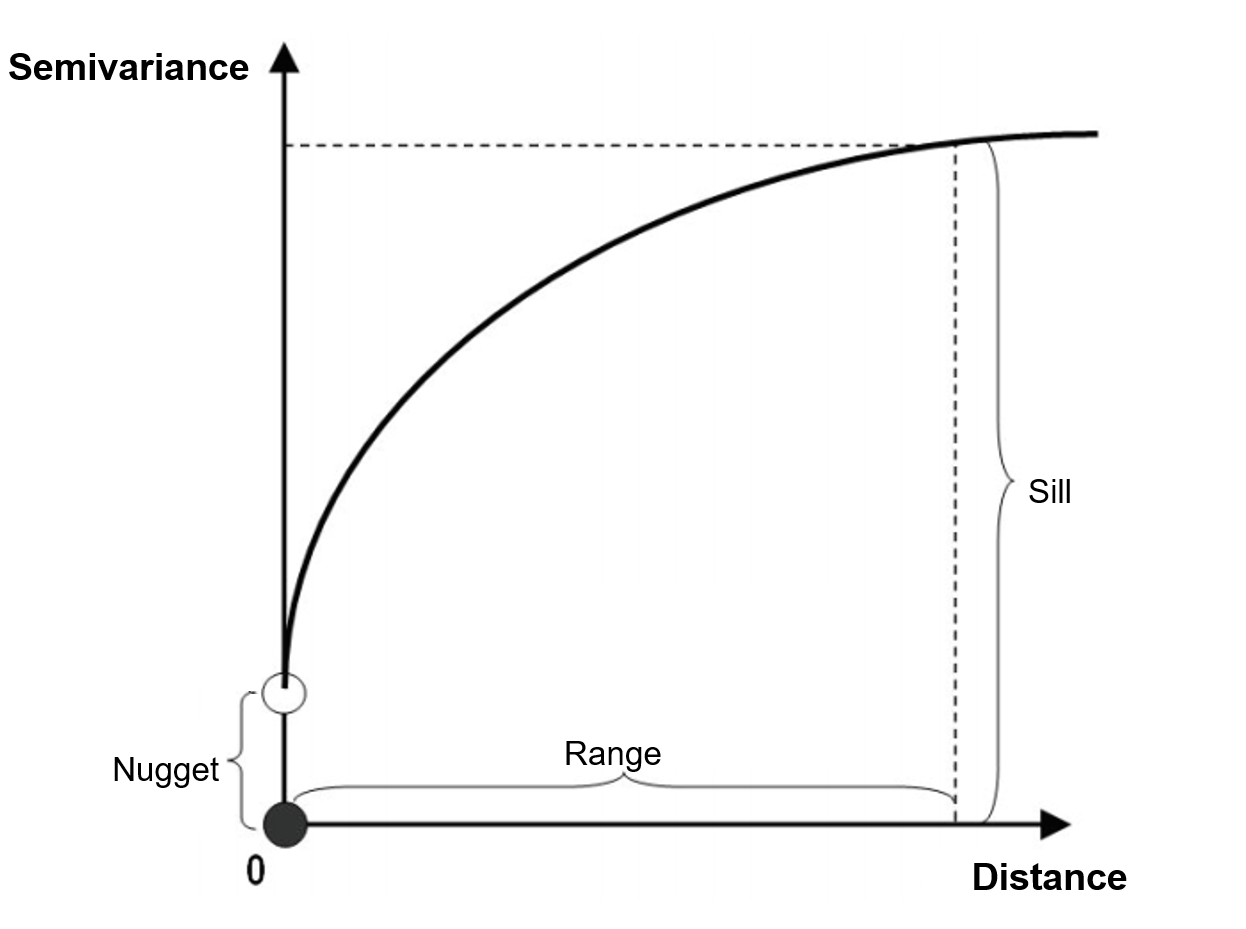
\includegraphics[width=0.6\textwidth]{./Images/variogram.png}
\caption{Example of a kriging variogram.}
\label{fig:variogram}
\end{figure}

\subsection{External Influences}

AERMOD and ADMS-urban are air pollution dispersion models that are reference standards for governments such as the ones of United States of America and United Kingdom for the precision modelling of air quality \cite{Mohan2011}.
AERMOD was developed at the United States Environmental Protection Agency and ADMS-Urban was developed by Cambridge Environmental Research Consultants. Both are used for regulatory purposes in the respective countries and highly recommended models in many other.

AERMOD is a gaussian plume air dispersion model which heavily takes meteorological and other external factors into account. The fact that it is plume based model, means that it considers the movement of one fluid through another, which in this case are the particles which move through the air. Some of the external factors which it takes into account are cloud cover observations, wind speed and direction, temperature, dew point,
humidity and sea level pressure. Meteorological data is accepted from multiple heights and wind, temperature and turbulence are treated as vertical profiles.

ADMS-Urban is a model of dispersion of pollutants released from industrial, domestic and road traffic sources in urban areas. This local Gaussian type model is nested within a trajectory model for areas within 50 km × 50 km \cite{Lee2013}.

These models recognize that air turbulence and dispersion are continuously variable, depending on height above ground, winds and temperature. Concerning the height above ground, virtually all airflow near the ground is neutral. Both models have steady state by nature, which means polluting gases conditions, between the time of emission and the time it reaches any receptor, do not change. Therefore, it is clear that plume models cannot be expected to give reasonable results for long range transport of pollutants.
Despite this, they can still be used to estimate pollutants concentration in areas where there is no monitoring stations, in the likes of interpolation methods \cite{Lee2013}.

In 2009, Mesquita, studied the performance of Multiple Linear Regression as an interpolation algorithm that uses external factors like city traffic emissions in comparison to the most common interpolation algorithms which do not encompass external factors, and this approach reflected notably better results than algorithms such as IDW and OK \cite{Mesquita2009}.


\subsection{Temporal Forecasting}

Zhang et al., in 2012, made a complete two part review of the history, techniques, current status of science and research and future prospects of real time air quality forecasting, where three major techniques for forecasting are distinguished \cite{Zhang2012} \cite{Zhang2012a}.

The simple empirical approaches, which are based on the assumption that today’s observed pollutant level is tomorrow’s forecasted value, are considered weak and of low accuracy. There are also parametric and statistical methods, which encompass regression methods and ANNs, and provide moderate to high accuracy. Finally, there are the advanced, physics based approaches, which are computationally expensive and complex and have very high operational costs and also have moderate to high accuracy \cite{Zhang2012}.

It is important to notice that for real time air quality forecasting, most methods are very circumstance dependent and regional related, with a big knowledge needed on the area subject to the forecasts.

Real time air quality forecasting does not belong to the scope of air spatial interpolation, therefore it will not be subject of study in this thesis but it could be considered for a prospect of future work for the developed systems.


\subsection{Practical Applications}

The above mentioned approaches have been developed and experimented both theoretically and empirically, with many of its applications documented in recent literature in the air pollution field.

A review of SIMs for environmental scientists made in 2008, by Li and Heap, theoretically compares 26 SIMs and concludes that the selection of an appropriate method for each different case is critical, but difficult, since its performance depends on the variable under study, the spatial configuration of the data and on the underlying assumptions \cite{Li2008}.

In 2013, Funenga, in his masters dissertation, used the OK interpolation method to infer the air quality related to polluting gases in the city of Lisbon, with the data available from the fixed monitoring stations \cite{Funenga2013}. The results showed poorly defined spatial continuity, since the interpolation only accepted inputs from 6 different stations, which represent very sparse data. Funenga also tested the Calpuff model for interpolation, which was, until 2017, the preferred system for the simulation of air pollution dispersion of the United States Environmental Protection Agency. This consisted of a model for the meteorological factors influence, a Gaussian puff dispersion model and a post-processing program for results output. In comparison to the OK, this model relative mean absolute error was lowered, which demonstrates high performance increase from the Calpuff method usage.

Tang et al., in 2017, proposed a spatial interpolation framework to incorporate diverse data sources and model the spatial processes explicitly at multiple resolutions with the use of spectral analysis and a spatial Gaussian process for interpolation, underlining the fact that when monitoring data sources are very sparse, auxiliary data should be added to the interpolation algorithms \cite{Tang2017}.

In 2018, Oteros et al., based on weather information, and on a kriging geospatial interpolation method, estimated daily pollen concentration in unmonitored areas, based on 26 monitoring stations in an area of approximately 71 000 km$^{2}$. It concluded, that the developed system was accurate enough for the spatial interpolation of pollen concentrations at unmonitored sites \cite{Oteros2018}.
Also in 2018, a study was conducted with the objective of proposing a low-cost mobile sensor network for evaluation of air quality in urban areas, with the use of kriging interpolation for data processing. It concluded that better results could have been taken if the modelling relied not only on measurements but also on spatial information such as weather data, building heights, and population density. It also confirmed that sparsely distributed sensor nodes, along with kriging interpolation, can be used to produce a real-time rendering air quality map \cite{Makowski}.

Machine learning techniques have also been incorporated into air quality interpolation, in order to improve its results and some of its processing and data constraints. 

Mishra et al., in 2015, used an artificial intelligence approach to forecast PM2.5 during haze episodes, compared Neuro-Fuzzy techniques with ANNs and Multiple Linear Regression, and concluded that its Neuro-Fuzzy model outperformed all the other approaches in the forecasting of PM2.5 \cite{Mishra2015}.

In 2018, Alimissis et al., evaluated both ANN and Multiple Linear Regression as interpolation methodologies, using data from a real urban air quality monitoring network of the concentration of different air pollutants in Athens, Greece. It was concluded that ANN were significantly better, especially where the monitoring network density was limited and there was consequently a low degree of correlation between the monitoring sites \cite{Alimissis2018}. Also in 2018, Franceschi et al. developed models to forecast particulate matter concentration using ANN, which were proven to be useful as references to issue early warnings of high air pollution in certain areas \cite{Franceschi2018}.

Measurement sensors are typically sparsely located, and that is one of the biggest problems to SIMs for the prediction of air pollution.

%In \Cref{fig:spatial-algorithms} are presented the models for %spatial air quality analysis, which are considered in this %work and will be tested in terms of overall performance for %an implementation as a live web visualization of the \ac{PM} %pollution in the city of Lisbon.

%\begin{figure}[h]
%\centering
%\includegraphics[width=1\textwidth]{./Images/spatial-algorithm%s.png}
%\caption{\ac{SIM}s considered in this work.}
%\label{fig:spatial-algorithms}
%\end{figure}

% #############################################################################
\section{LPWAN Technologies}

Small devices with \ac{CPU}, memory, sensors and capable of mobile communications through which they can connect to the internet have a great potential to change our society. The inter-networking of these devices is called IoT. Data collected can be shared and analyzed in real time through the Internet. These objects and networks can help improve society and its citizens lives in many different ways.

In fact, the number of devices connected to the Internet has seen a big growth in the recent years and is expected to keep growing exponentially, as people increase the devices they purchase. This growth is unprecedented in the communication industry as well as in the wider global economy. It is estimated that by 2020, more than 50 billion devices will be connected through radio communications \cite{Holler2014}.

IoT has seen various applications in many practical research fields, due to specific requirements such as long range, low data rate, low energy consumption and cost effectiveness.

The most widely used radio technologies nowadays are either short-range technologies such as Zigbee, Bluetooth and Wi-Fi (which are not suited for scenarios that require long-range transmission), or cellular communication technologies, such as 2G, 3G and 4G (which provide long-range access but have excessive power consumption) \cite{Mekki2018}. With this gap in the radio communications and the emerging IoT technologies, increasing number of devices and many useful practical application projections, a new group of technologies was developed so that long-range transmission could be provided with low consumption and communication costs, named LPWAN \cite{Mekki2018}. This group of technologies is considered to be ideal for the research to be developed in this work, with its application to the system that will be produced. It can be used since a low data rate is allowed, and long-range access together with low-consumption are needed.

LPWAN represents the current trend in the evolution of IoT technologies as it is increasingly gaining popularity both in industrial and research environments, due to its low production and consumption costs. In order to achieve these specifications, usually a small data rate limitation is imposed. LPWAN technologies are an excellent choice for long-term monitoring applications in urban areas, as can be seen by its advantages in \Cref{fig:ieec4}.

Until the appearance of LPWAN technologies, the two main approaches to IoT were multi-hop mesh networks with short-range technologies in the unlicensed spectrum or long-range conventional cellular technologies such as GSM and \ac{GPRS} \cite{Zanella2016}. Experimental trials made by Zanella et al. in 2016 allowed the conclusion that by using LPWAN technologies, less than half of the gateways are needed to cover the same urban area than the number of sites deployed by one of the major cellular operators in Italy, to provide mobile cellular access.

Currently, there are several LPWAN technologies being used both for research and business applications. The most popular and suitable for this work are SigFox, \ac{LoRaWAN}, \ac{LTE-M} and NB-IoT. While SigFox and LoRaWAN are proprietary technologies, operating in the unlicensed spectrum, LTE-M and NB-IoT are standardized by \ac{3GPP} and operate in the licensed spectrum. In this section, an overview of these technologies is made, as well as a comparative analysis regarding related empiric studies in the literature and the characteristics that differentiate them from each other.

The business and commercialization application of LPWAN is already taking place. A survey on LPWAN technologies, made in 2017, stated that the successful implementation of LPWAN technologies such as NB-IoT and LoRaWAN had already been started in North America and Europe. Meanwhile, several mobile operators in countries like Korea, Japan and China, according to the survey, also already had plans to implement nationwide NB-IoT or LoRaWAN \cite{Sinha2017}. 

In Portugal, the mobile operator Altice Portugal has announced total NB-IoT coverage in Portugal by the beginning of 2019 \cite{Altice2018}. 

The rest of the LPWAN technologies have the following coverage in Portugal, at the time of this thesis: SigFox has full coverage, according to its website \cite{SigFox2018}; LoRaWAN has decent coverage, available through a total of 43 gateways implemented throughout the country by several communities in Portugal \cite{ThingsNetwork2019}; there is currently no record of any LTE-M implementation. 

\begin{figure}[ht]
\centering
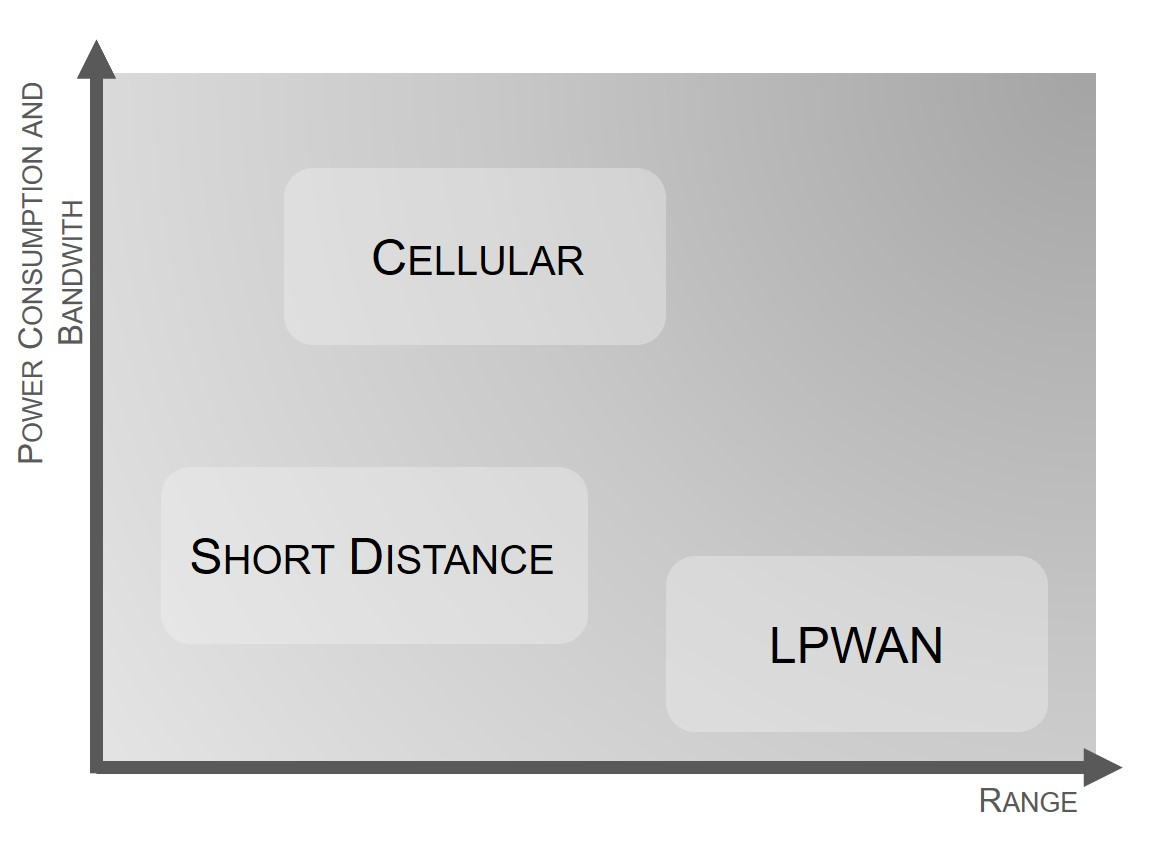
\includegraphics[width=0.6\textwidth]{./Images/ieec4.jpg}
\caption{Comparison of LPWAN with other technologies.}
\label{fig:ieec4}
\end{figure}

\subsection{SigFox}

The SigFox physical layer employs \ac{UNB} wireless modulation, and its network layer protocols are proprietary. Bidirectional communication is supported and SigFox claims that each gateway can handle up to a million connected objects, with a coverage area of 30 to 50 km in rural areas and 3 to 10 km in urban areas.

The ultra-narrow-band technology has communication channels with approximate bandwidth of 100Hz, uplink-triggered transmissions that follow a client-server model and cooperative reception from multiple gateways. An end device wakes up only when uplink data arrives, and then randomly selects a channel for uplink transmission, which is repeated three times to increase the chances of a successful reception by the network. Following this uplink transmission, for the next 10s, there is the possibility for receiving a downlink message on a predetermined channel \cite{Yang2017}.

\subsection{LoRaWAN}

LoRaWAN is another popular LPWAN solution, patented by Semtech Corporation. It has a proprietary \ac{PHY}, \ac{LoRa}, but the rest of the protocol stack, designated LoRaWAN, is open. LoRaWAN networks, like SigFox, typically have a star topology with many end devices connected by a single-hop link to gateways, which are connected to a common network server via standard IP protocols, with its gateways
being totally transparent to end devices, providing simpler network management.

LoRaWAN supports 3 types of end devices, each type characterized as a class. Class A supports bidirectional communications through, right after uplink transmission, two short period downlink receive windows. This class has the lowest power consumption, but like SigFox, for downlink transmission, servers need to wait for the next scheduled uplink transmission. Class B devices are also bi-directional, but with scheduled receive slots, and Class C devices have maximum receive slots, which offer the lowest latency for server to device communications in all the classes, but the most power consumption as well.

In order to maximize a device battery and overall capacity, the communication bandwidth is managed by the LoRaWAN network, for each device, which does not happen with SigFox, where the bandwidth is fixed. The LoRa modulation is proprietary and is based on chirp spread spectrum to increase the immunity to interference in the unlicensed bandwidth \cite{LoRaAlliance2017}.

\subsection{LTE-M}

LTE-M, also known as \ac{LTE} Cat M1, \ac{LTE-MC} or \ac{eMTC}, is a standardized LPWAN technology, by 3GPP, which operates in the licensed spectrum. It has the same design of LTE, regarding transmission structure, downlink \ac{OFDMA}, uplink \ac{SC-FDMA} and same channel coding as well. In order to reduce the cost and power consumption in comparison to LTE, technologies like reduced peak rate, simplified hardware and narrow band operation were implemented \cite{Yang2017}.

As such, LTE-M has the LTE minimum system bandwidth of 1.08 MHz and the minimum communication bandwidth of 180 kHz per device. This is considered to be wasteful in terms of spectral efficiency and also prevents the deployment in narrower cellular bands like GSM legacy cellular services bands, which have increasingly been re-farmed for new wireless services. It also raises the problem of lack of support to the upcoming industry massive IoT, considering the scarce spectrum \cite{Yang2017}.

\subsection{NB-IoT}

NB-IoT, also known as LTE Cat NB1, is also a LPWAN technology standardized by the 3GPP, created in 2015 to face the growing massive IoT connectivity challenge, targeting the exploitation of the re-farmed GSM spectrum. It operates on 180 kHz bandwidth (same as LTE bandwidth per device) for both downlink and uplink. The downlink remains with the same structure as LTE (OFDMA with 15 kHz
subcarrier spacing), and the uplink is SC-FDMA with sub-carrier spacing at 3.75 kHz (15 kHz for in-band to avoid interference from other LTE traffic), which is also the minimum transmission bandwidth for a device \cite{Ratasuk2016}.

The advantages of NB-IoT are its enhanced indoor coverage, the ability to connect a massive number of low-throughput devices, but with a lower data rate. Its main objectives include low-cost devices, high coverage, long device battery life, and massive capacity, with some relaxation in latency.

The NB-IoT network is designed to work seamlessly on existing GSM and LTE networks within the licensed frequency bands, making use of the already deployed mobile operator’s base stations. Due to this, currently many telecommunication manufacturers are supporting the standardization of the NB-IoT network \cite{Song2017}.

A literature analysis regarding empiric and review studies which contain comparisons between the IoT technologies was made. In 2016, Centenaro et al. conducted a LoRaWAN deployment test in Northern Italy, from which it was concluded that the LPWAN paradigm has the potential to complement current IoT standards as an enabler of smart city applications, since with LoRaWAN, the gateways needed to cover
a certain area are considerably less than the base stations a cellular operator would need to cover the same area. A study by Yang et al. in 2017, which analyzed and compared the effective bandwidth of SigFox, LoRa, LTE-M and NB-IoT, concluded that it is yet too early to say which is the best technology, since there still remain many challenging issues waiting for solutions in the area. A \ac{MAC} layer-based evaluation with the use of a probabilistic model, concluded that NB-IoT is more robust that both LoRaWAN and SigFox in terms of Packet Error Rate \cite{Mroue2018}.

In a study by Ikpehai et al. in 2018, through the specifications analysis and a network simulation scenario of several LPWAN technologies, it was concluded that LoRaWAN offers the longest range, LTE-M has the higher power consumption, and NB-IoT provides the widest coverage, since it is supported by mobile operators, while LoRaWAN gateways are private and sparsely scattered. A study by Lauridsen et al. in 2017, through a coverage comparison of GPRS, NB-IoT, LoRaWAN, and SigFox in a 7800 km area, using a 3GPP Rural Macro and Urban Macro non-line-of-sight model simulation in a realistic scenario, also concluded that from the LPWAN technologies NB-IoT is the one that provides the best coverage, even in indoor scenarios \cite{Ikpehai2018}.

Other interesting conclusions also were that both SigFox and LoRaWAN are better when the amount of data that must be sent daily is beneath 1000 bytes, while NB-IoT is more suitable for cases where this number is between 1000 and 10000 bytes, since it maintains its extended device lifetime in these situations \cite{Finnegan2018}. A survey specifically on LoRaWAN and NB-IoT technologies concluded that LoRaWAN is more suitable for industrial applications, while NB-IoT is better to personal and public applications \cite{Zanella2016}.

The analysis to the specifications of all the LPWAN technologies mentioned, as well as conclusions attained from the reviewed literature, are presented in \Cref{table:LPWAN}, which is inspired in the listed characteristics by Yang et al., in 2017 \cite{Yang2017}, and summarizes the analysis made in this section.

% TODO: rectificar tabela = centrar verticalmente

%\renewcommand{\tabcolsep}{3pt}
\renewcommand\arraystretch{2}
\begin{table}[ht]
\centering
\caption{LPWAN technologies comparison.}
\label{table:LPWAN}
\begin{tabular}{m{0.115\textwidth}>{\centering}m{0.17\textwidth}>{\centering}m{0.2\textwidth}>{\centering}m{0.115\textwidth}>{\centering\arraybackslash}m{0.25\textwidth}}
\toprule
&SigFox&LoRaWAN&LTE-M&NB-IoT\\
\midrule
Receiver Sensitivity&-147 dBm&-147 dBm&-132 dBm&-137 dBm\\
Frequency Band&Sub-GHz ISM&Sub-GHz ISM&Licensed&Licensed\\
Minimum Transmission Bandwidth&100 Hz&125 kHz&125 kHz&3.75 kHz\\
Modulation&D-BPSK&LoRa proprietary modulation, GFSK&BPSK, QPSK, 16QAM& $\pi \div 2 – \textrm{BPSK}, \pi \div 4 – \textrm{QPSK}$ \\
MAC & Unslotted ALOHA & Unslotted ALOHA & SC-FDMA & SC-FDMA \\
Over the air updates& No & Yes & Yes & Yes \\
Related Work & Suitable when data to be sent daily is beneath 1000 bytes \cite{Finnegan2018}.& Suitable to IoT industrial applications \cite{Sinha2017} and when data to be sent daily is beneath 1000 bytes \cite{Finnegan2018}; Longest range \cite{Ikpehai2018} & Most heavy power consumption \cite{Ikpehai2018}.& Suitable to IoT personal and public applications \cite{Sinha2017} and when data to be sent daily is between 1000 and 10,000 \cite{Finnegan2018}; Widest coverage \cite{Ikpehai2018}\cite{Lauridsen2017}; The most robust, considering the Packet Error Rate \cite{Mroue2018}.\\
\bottomrule
\end{tabular}
\end{table}%

%\begin{table}[htb]
%\centering
%{
%    \caption{LPWAN technologies comparison.}
%    \label{tab:LPWAN}
%    \begin{tabular}{ | c | c | c | c | c |}
%    \hline
%   & SigFox & LoRa & LTE-M & NB-IoT \\
 %   \hline \hline

 %   Receiver & -147 dBm & -147 dBm & -132 dBm & -137 dBm \\
 %   Sensitivity &   &   &   & \\
    %\textbf{Protocol} & & & \\ 
  %  \hline
    
  %  Frequency & Sub-GHz & Sub-GHz ISM & Licensed & Licensed \\ 
  %  Band & ISM & & & \\
    %\textbf{Codec} & &  & \\ 
 %   \hline
    
%    Minimum & 100 Hz & 125 kHz & 125 kHz & 3.75 kHz \\
%    transmission &  &   &   & \\
%    bandwidth &   &   &   &   \\
    %\textbf{Codec} & & & \\ 
%    \hline
    
 %   Modulation & D-BPSK & LoRa proprietary & BPSK, QPSK, & \\
 %    &  & modulation, GFSK & 16QAM & $\pi \div 2 – BPSK, \pi \div 4 – QPSK$ \\
%      &   &   & 16QAM & \\
    %\textbf{Format} & F4V & & \\ 
%    \hline
    
%    MAC & Unslotted ALOHA & Unslotted ALOHA & SC-FDMA & SC-FDMA \\
 %    & ALOHA &  &  & \\
 %   \hline
    
%    Over the air updates& No & Yes & Yes & Yes \\
 %   updates &  &  &  & \\ \hline
    
%    Related Work & Suitable & Suitable to IoT industrial & Most heavy & Suitable to IoT personal and \\
 %    & when data & applications \cite{Sinha2017} and & power & public applications \cite{Sinha2017} and \\ 
 %    & to be sent & when data to be sent & consumption & when data to be sent daily is \\
 %    & daily is & daily is beneath 1000 & \cite{Ikpehai2018} & between 1000 and 10,000 \\
%     & beneath & bytes \cite{Finnegan2018}; Longest &  & \cite{Finnegan2018}; Widest coverage \\
%     & 1000 bytes & range \cite{Ikpehai2018}. &  & \cite{Ikpehai2018}\cite{Lauridsen2017}; The most robust, \\
%     & \cite{Finnegan2018}. &  &  & considering the Packet Error \\
%     &  &  &  & Rate \cite{Mroue2018}. \\
%    \hline
%    \end{tabular}
%    }
%\end{table} 


% #############################################################################
\section{IoT Hardware Solutions}

In March of 2018, Rahman et al. developed and implemented an IoT based platform for developing cities aimed at environmental monitoring. For this project, 3G cellular connections were used, due to the lack of availability of other low-cost radio technologies. This system was composed of an Arduino Nano micro-controller to retrieve the data from the gas sensors, and a Raspberry Pi to store and process that data, which is then stored and sent through 3G to the cloud \cite{Rahman2018}.

In fact, throughout the literature, many IoT solutions produced for research purposes use single board computers such as Raspberry Pis as the core data processing unit, as well as micro-controllers such as Arduinos. These devices are popular research tools in the development of IoT systems in areas such as healthcare, smart home automation, smart agriculture and environment monitoring \cite{Rahman2018}. 

In recent literature, there are examples of the use of Raspberry Pis as core systems in air quality monitoring research. Ibrahim et al. developed, in 2015, an IoT Smart Monitoring system using a Raspberry Pi, to process and send the data received to the cloud. In 2016, both Shete et al. and Balasubramaniyan et al. developed a similar system to monitor climate data also with the use of a Raspberry Pi \cite{Shete2016} \cite{Balasubramaniyan2016}. These projects have the limitations of having a relatively high power consumption and the need to use Wi-fi for the Internet access. In 2017, Patil et al. developed a system for the smart monitoring of the air quality also based on a Raspberry Pi. This project was developed using the wireless communication protocol Zigbee and an Arduino micro-controller \cite{Patil2017}.

Both Raspberry Pis and Arduino based devices are reliable products to be used in IoT systems. Raspberry Pi is a single board computer, running an operating system. An Arduino based micro-controller is simpler, with much lower memory and processing power, and can only run one program at a time. This results in a higher energy consumption and cost in the Raspberry Pi, and the opposite in comparison to Arduino based micro-controllers. However, in terms of processing power and data storage, the Raspberry Pi is dominant, since Arduino has less memory and processing power \cite{Balasubramaniyan2016}.

It can be concluded that Raspberry Pis are suitable for heavy duty situations such as, in the air quality monitoring systems scope, the processing and storage of a large amount of data from many sensors. On the other hand, an Arduino based micro-controller would be suitable for a simpler implementation with only one or two sensors and a simple data retrieval and processing mechanism.

Currently, NB-IoT technologies are in early stages of availability, but there are already several solutions provided by the industry for its hardware implementations in the form of Arduino based boards. Main manufacturers of NB-IoT chipsets and modules include Huawei, Intel, QualComm, Samsung, Nordic Semiconductor, Sierra Wireless and U-Blox, and many of these solutions are already being implemented in business domain applications \cite{Yllasjarvi2018}.

Despite this, a relevant application of this technology to air quality monitoring systems could still not be found in the literature, providing this work an opportunity to enlighten some information on this area and provide useful conclusions regarding this technology implementation in a low cost and consumption air quality monitoring system.


% #############################################################################
\section{Air Pollution Visualization}

Air pollution visualization is one of the objectives of this thesis. Research was made in order to find the current forms of public presentation of live information regarding the air quality in parts of the world where there are enough monitoring stations for it to be possible.
Currently there are two types of platforms for the visualization of live air quality data: the governmental platforms and the private companies platforms.

\begin{figure}[ht]
\centering
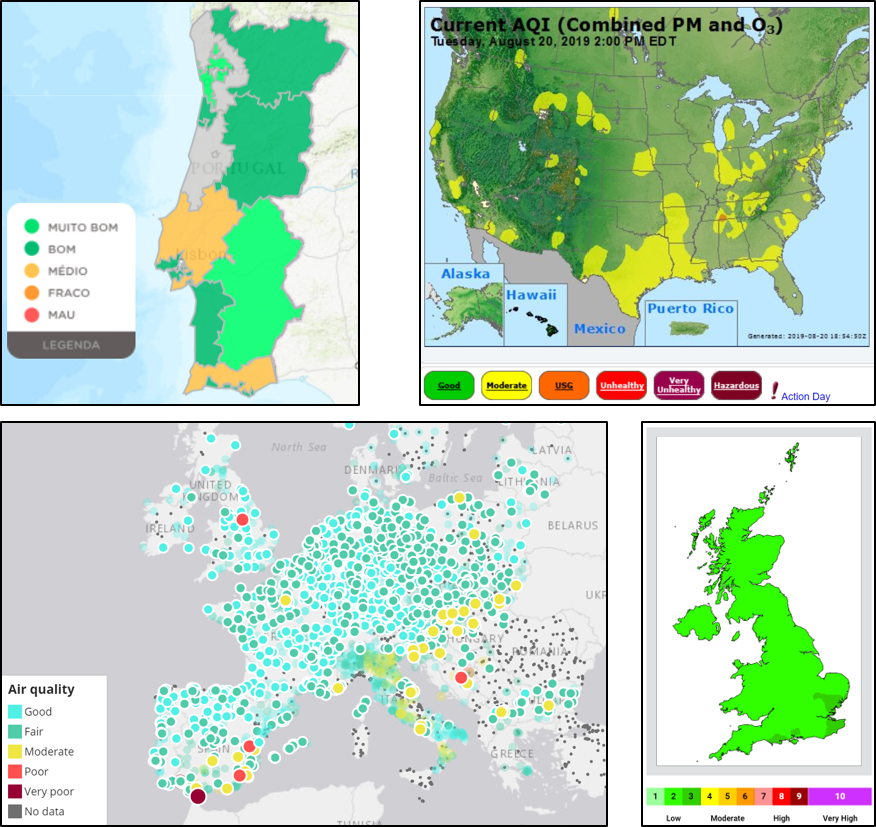
\includegraphics[width=0.65\textwidth]{./Images/air-visualization.png}
\caption{Governmental public online platforms for live air quality visualization.}
\label{fig:air-visualization}
\end{figure}

Reviewed governmental platforms in Europe and America, do not show fine interpolated data in their air quality maps. They only present, for each individual monitoring station, its local air quality index value. This leads to low resolution maps which are difficult to perceive and do not show air quality variances between stations. Some of these governmental platforms are presented in \Cref{fig:apa-stations-location}. At the top left is the QualAr platform, at the top right is the United States Environment Protection Agency one, at the bottom right is the air visualization provided by EEA, and at the bottom right is the platform provided by the United Kingdom government \cite{QualAr}\cite{U.S.EnvironmentProtectionAgency}\cite{EEA}\cite{DepartmentforEnvironment}.


Air quality visualization platforms from external companies to the government are business oriented and take advantage of the publicly available air quality data provided governments to make their live interpolated air pollution map as a product. Examples of these are Breezometer and AirVisual. These present heat maps with a much finer resolution than the ones provided by governments, as can be seen in \Cref{fig:breezo-visualization} \cite{Breezometer}. However, the spatial modelling algorithms used for the interpolation are proprietary, are not open-source and do not contribute to the literature, which is the aim of this work. Additionally, the accuracy provided from these is only extended to 500 meters \cite{Breezometera}.

\begin{figure}[ht]
\centering
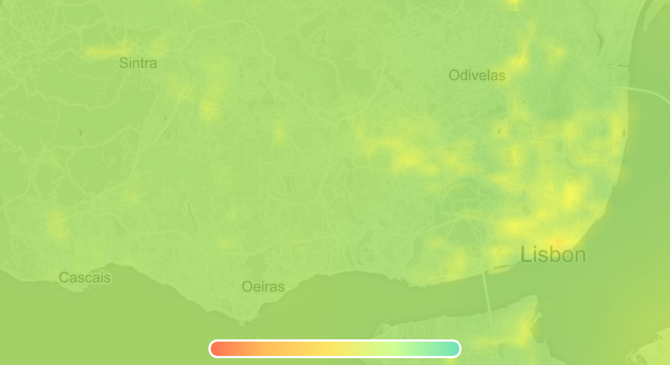
\includegraphics[width=0.6\textwidth]{./Images/breezo-visualization.png}
\caption{Breezometer high resolution live air quality map.}
\label{fig:breezo-visualization}
\end{figure}


%ler: https://blog.breezometer.com/accurate-air-quality-data
% https://blog.breezometer.com/understanding-air-quality-data
    
% #############################################################################